\documentclass[]{article}
\usepackage{graphicx}

\title{HPC-Master.Lab4}
\begin{document}
\maketitle

\setlength{\parindent}{0pt}
\setlength{\parskip}{3pt}

\section{Introduction}
In this labwork, I implemented the image grayscale function with GPU acceleration with 2D block size.
There will be 2 comparisons, presented in the sections below, one varied block sizes and with 1D block size implementation from the previous labwork

\paragraph{Source Image}
The image file from the previous labwork is reused. But similarly to the "varied block size comparisons" section of the previous report, some upscaling must be done to see considerable difference.
In the previous one I import the $cv2$ library and use the $cv2.resize$ method but that one is slow due to the interpolations, so in this labwork, i simply just repeat the image pattern using $numpy$, as the code follows:
\begin{verbatim}
SCALE = 7
hostSrc = np.hstack([
    np.vstack([
        hostSrc for _ in range(SCALE)
    ])
    for _ in range(SCALE)
])
\end{verbatim}

\paragraph{Code Implementation}
Below is the 2D version of the GPU accelerated image grayscale function. So pretty much identical to the 1D implementation, with the additional of $tidy$ for the location in the additional dimension. I also made the tuple $(tidx, tidy)$ and unpack them in the index reference just to avoid repetition.
\begin{verbatim}
@cuda.jit
def gpu_grayscale(src, dst):
  tidx = cuda.threadIdx.x + cuda.blockIdx.x * cuda.blockDim.x
  tidy = cuda.threadIdx.y + cuda.blockIdx.y * cuda.blockDim.y
  tid = (tidx, tidy)
  g = np.uint8((src[*tid, 0] + src[*tid, 1] + src[*tid, 2]) / 3)
  dst[*tid, 0] = dst[*tid, 1] = dst[*tid, 2] = g
\end{verbatim}

\section{Varied Block Size Comparison}
For the block sizes choice, I still go with the power of 2s. But since the limit is $(32, 32)$, I only get the permutations of the values $(8, 16, 32)$, which results in 9 values in total.
The execution is repeated for $30$ times then takes the average time, below is the comparison graph

\begin{figure}[h]
    \centering
    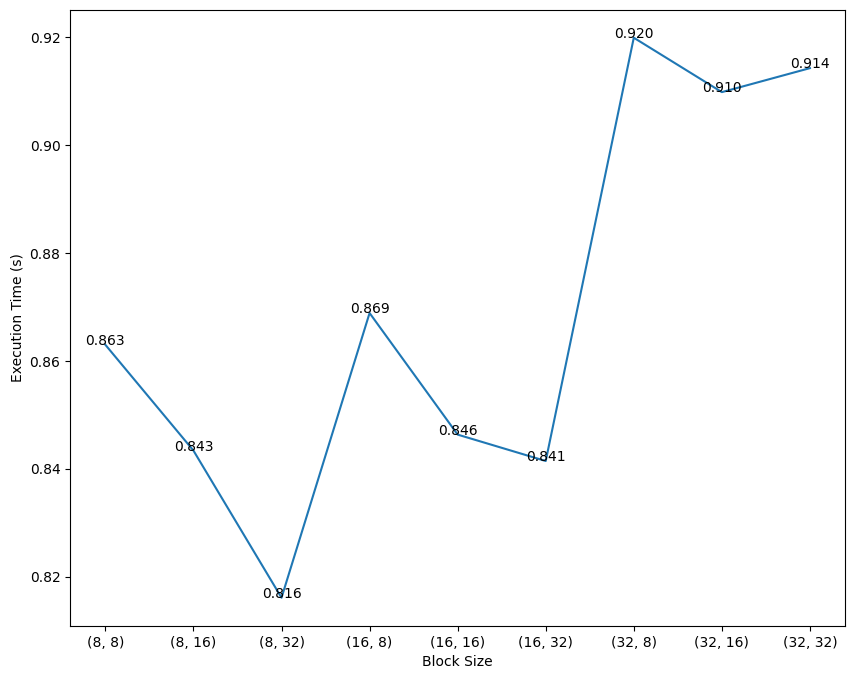
\includegraphics[width=0.75\linewidth]{blocksizes-compare.png}
    \caption{Block Sizes Comparison}
    \label{fig:blocksizes-compare}
\end{figure}

So increasing the \textbf{y} block size seems to helps the execution faster. And in contrary, increasing \textbf{x} block size decrease the performance.
The can be observed as $(8, 32)$ is the best block size configuration while $(32, 8)$ is the worst.
Unfortunately I cannot think of an explanation for this result.

\section{1D Program Comparison}
To compare with the 1D program made in the previous labwork, I keep the same block size of $64$ for that 1D program, and set the block size $(8,8)$ for the 2D program, this makes it fair in terms of number of threads per block.
The run block of the 1D program add the flattening and reshaping steps compare to the previous labwork. 
The execution is repeated for $30$ times then takes the average time, and here is the result
\begin{itemize}
\item \textbf{1D}: $\approx 0.827s$
\item \textbf{2D}: $\approx 0.878s$
\end{itemize}
So the 1D program is faster although the 2D program is more natural to visualize and despite the additional steps of flattening and reshaping.

\end{document}